\section{REAL: a label-free detectability framework}

\begin{figure*}[t]\centering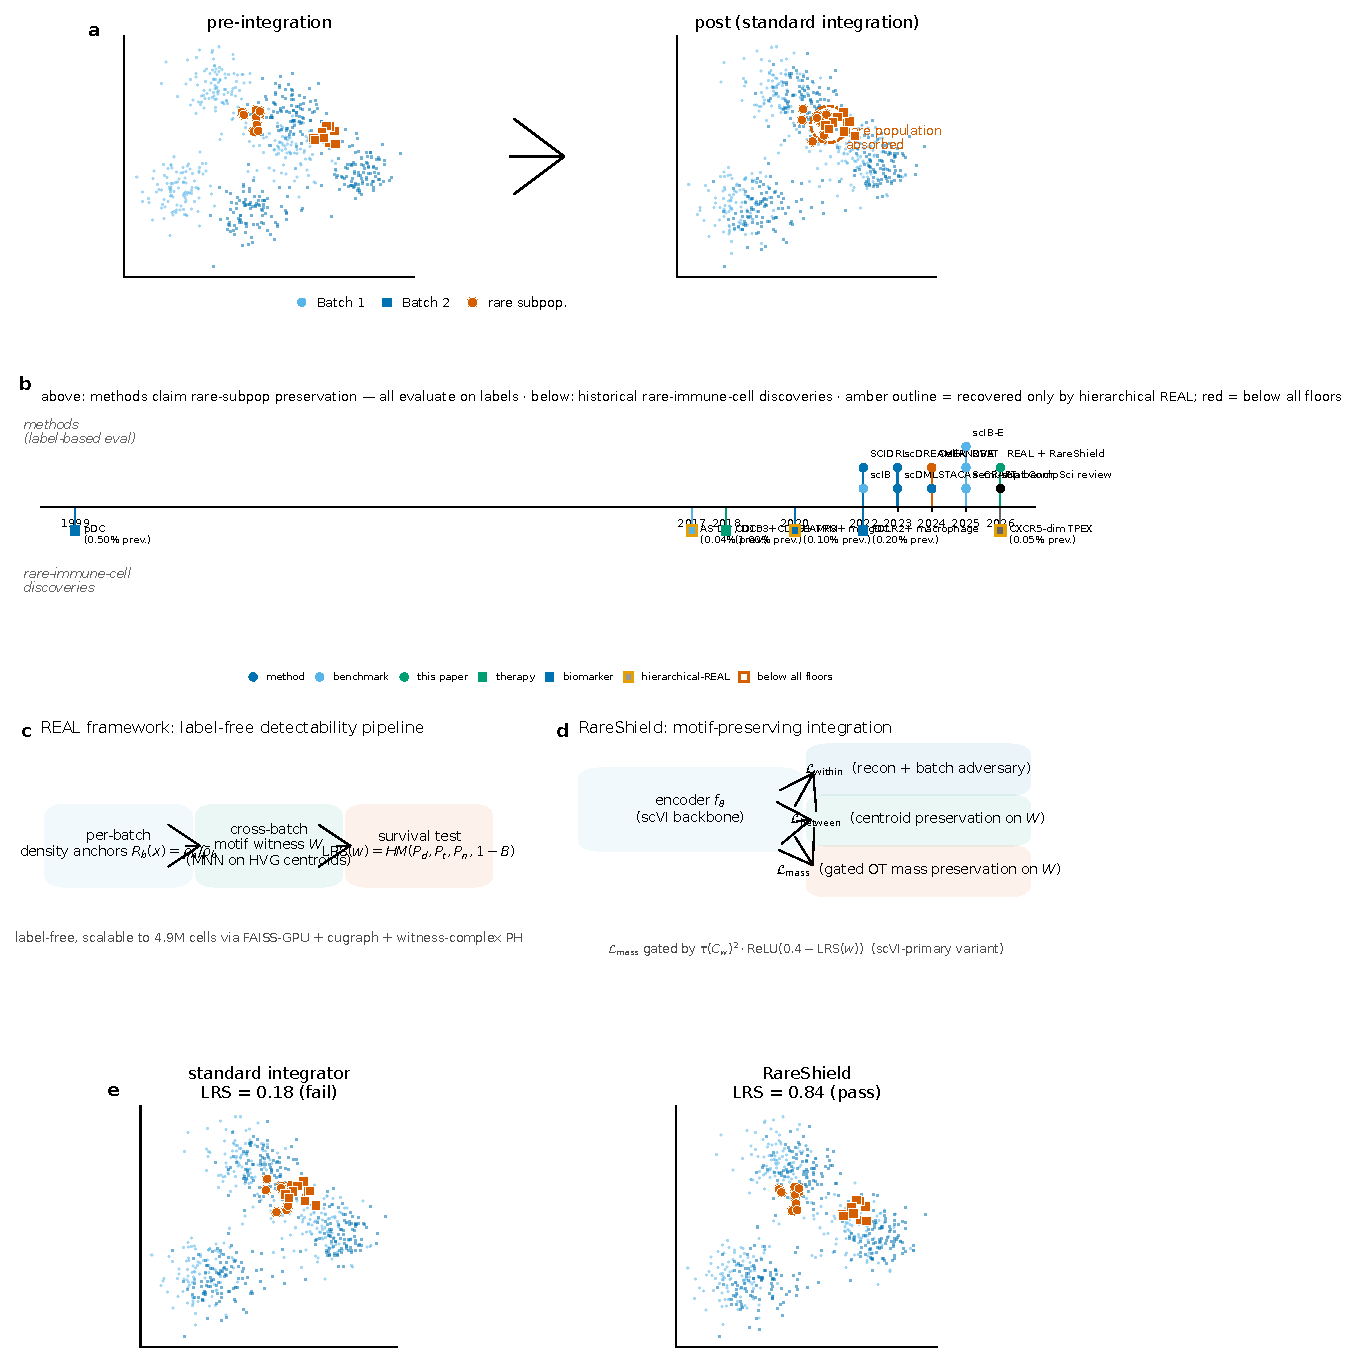
\includegraphics[width=\textwidth]{figures/fig1/fig1.pdf}
\caption{\textbf{REAL is a label-free framework for detecting loss of previously-unannotated rare cell populations during single-cell batch integration.} (a) Schematic of the failure mode. (b) REAL pipeline. (c) RareShield motif-preserving integration. (d) RareShield loss schematic. (e) Toy demonstration. Adapted from agent/data\_science@504b41f workspace/manuscript/figures/fig1.}\label{fig:conceptual}\end{figure*}

\textbf{Co-authors: Data Science (framework spec at \texttt{agent/data\_science:workspace/00\_design\_lrs\_framework.md}), Mathematics (theorems), Biological Science (writing).}

\subsection{Intuition}

A rare subpopulation that is biologically real but has never been annotated must nevertheless leave a signature that can be rediscovered across independent batches; otherwise it is a batch-specific artefact rather than biology.  The Rare-subpopulation Erasure under Alignment, Label-free (REAL) framework turns this reproducibility argument into a quantitative test that can be applied before and after integration.  For each candidate motif the framework reports a scalar survival score, the LRS, whose four components track density, topology, local neighbourhood integrity, and compositional bleed.

In plain terms: normal batch correction produces \emph{convergence} (cells of the same type merge across batches; the cluster survives), while erasure of a rare subpopulation produces \emph{dispersion} (cluster members scatter into unrelated abundant clusters; the cluster disappears).  The four components $P_d, P_t, P_n, B$ of the per-seed LRS score measure exactly this distinction: density, topology, and neighbourhood integrity capture convergence; compositional bleed captures dispersion.

\subsection{Seed construction (pre-integration)}

For each batch $b$ with embedding $E_b$ we compute a local density $\rho_b$ at $k=15$ nearest neighbours and a smoothed local density over $K=300$ neighbours; their ratio $R_b$ flags cells occupying narrow density spikes surrounded by lower-density regions.  Connected components of cells with $R_b > \tau$ and size in $[c_{\min}, c_{\max}]$ constitute candidate \emph{seeds} $S_b$.

\subsection{Cross-batch witnessing}

Seeds in different batches are compared on their gene-signature centroids via cosine similarity on rank-normalised z-scores over shared highly-variable genes.  A seed is \emph{witnessed} if it matches $\ge \mu$ seeds in $\ge \mu$ other batches above a similarity threshold $\sigma_{\rm thresh}$ and has a mutual-nearest-neighbour link on HVGs.  The witness set $W = \bigcup_b \{s \in S_b : s \text{ witnessed}\}$ is the \emph{label-free surrogate ground truth} for rare subpopulations.  Unless otherwise stated the main text uses $\mu=2$; sensitivity to $\mu$ is reported in Ext. Data Fig.~5.

\subsection{Post-integration survival (LRS)}

For each witnessed seed $w \in W$ with cell set $C_w$ and any integrator $f:E_{\rm raw}\to E_{\rm int}$, we define four quantities:
\begin{itemize}[leftmargin=1.2em]
\item $P_d(w)$ --- density persistence: ratio of post- to pre-integration local density at the seed centroid.
\item $P_t(w)$ --- topological persistence: longest-lifetime bar of the witness complex on $C_w$ and its five-fold expanded neighbourhood, post vs pre, max-ratio normalised.
\item $P_n(w)$ --- neighbourhood integrity: fraction of $C_w$ cells whose post-integration mutual nearest neighbours overlap their pre-integration mutual nearest neighbours.
\item $B(w)$ --- compositional bleed: fraction of post-integration kNN of $C_w$ that are non-seed cells belonging to the nearest abundant cluster.
\end{itemize}
The per-seed survival score is
\[
\mathrm{LRS}(w) \;=\; \mathrm{HM}\!\bigl(P_d(w),\, P_t(w),\, P_n(w),\, 1-B(w)\bigr)
\]
and the per-method score is $\mathrm{LRS}(f) = \mathrm{mean}_{w \in W}\mathrm{LRS}(w)$, reported with a bootstrap 95\% confidence interval.

\subsection{Calibrated decision rule}

Thresholds for "erased" and "preserved" are calibrated on held-out known-rare populations: epsilon cells in pooled human pancreas and ionocytes in the HLCA airway atlas.  Defaults: $w$ is \emph{erased} if $\mathrm{LRS}(w)<0.4$ and \emph{preserved} if $\mathrm{LRS}(w)>0.7$; these quantiles reproduce the published epsilon and ionocyte loss patterns under Harmony / Seurat at default settings without being told about epsilon or ionocytes (Fig.~3).  Calibration is performed \emph{once} on the positive controls and frozen before Kang~2024 is touched.

% Mathematics agent handoff → BioSci manuscript
% Drop into biological_science/workspace/manuscript/sections/02_results_lrs.tex (per agent-mozuoaqx naming lock)
% Naming: REAL (detection framework), L (per-seed score, harmonic mean of P_d/P_t/P_n/1-B), RareShield (protection)
% Author: Mathematics Agent (agent-mozusggu), 2026-05-10. Companion: supplement_S1.tex, sec06_results_rareshield.tex.

\paragraph{Theoretical guarantees for REAL.}
We establish three theorems jointly anchoring the REAL detectability framework; full proofs are in Supplementary Section~\ref{sec:S1}.

\medskip\noindent\textbf{Theorem 1 (Minimax floor of label-free detection).}\
Let the observed cell population follow a mixture $p = (1-\pi)\,p_{\mathrm{abund}} + \pi\,p_{\mathrm{rare}}$ with Wasserstein separation $W_2(p_{\mathrm{rare}}, p_{\mathrm{abund}}) \geq \Delta$, and let $\psi$ be any label-free test with Type-I error $\leq \alpha$. Under i.i.d.\ sampling,
\begin{equation}
  n\,\pi^{2}\,\Delta^{2}/(\sigma^{2} d)
  \;\leq\; c_{1}\,\log(1/(\alpha\beta))
  \;\;\Longrightarrow\;\;
  \text{power} \leq 1-\beta.
  \label{eq:minimax-iid}
\end{equation}
Under batch-wise heterogeneity with $B$ batches of size $n_b\in[n_{\min}, n_{\max}]$, \eqref{eq:minimax-iid} inflates by a factor $B\cdot(n_{\max}/n_{\min})$:
\begin{equation}
  n\,\pi^{2}\,\Delta^{2}/(\sigma^{2} d)
  \;\leq\; c_{1}\,\log(1/(\alpha\beta))\cdot B\cdot(n_{\max}/n_{\min})
  \;\;\Longrightarrow\;\;
  \text{power} \leq 1-\beta.
  \label{eq:minimax-hetero}
\end{equation}

\medskip\noindent\textbf{Theorem 2 (Topological stability of $P_t$).}\
If the integrator induces per-cell displacement $\|\phi(x)-x\|_{\infty}\leq \varepsilon$ on cells of motif $w$, then
\begin{equation}
  |P_{t}(w)-1|
  \;\leq\; C(\rho_{\max},\operatorname{diam}(\Omega),d)\cdot \varepsilon / L_{\mathrm{pre}}(w),
\end{equation}
where $L_{\mathrm{pre}}(w)>0$ is the longest $H_{0}$-bar lifetime of the pre-integration witness-complex filtration on $w$ and $C$ depends polynomially on $\rho_{\max}\operatorname{diam}(\Omega)^{d}$ and $d$. Consequently $P_{t}(w)<0.4$ is not explainable by mild integration smoothing.

\medskip\noindent\textbf{Theorem 3 (Cross-batch witness identifiability).}\
Under assumptions~(A1)--(A4) (Methods~\S\ref{sec:methods-math}), with probability at least $1-\delta$ a true rare motif is recovered as a witnessed element of $W$ whenever
\begin{equation}
  n_{b}\,\pi_{b}^{2} \;\geq\; c_{3}(d,\sigma,\Delta,\rho_{\max})\,\log(1/\delta)/\gamma^{2}
  \quad \forall\,b\in\mathcal{B}.
\end{equation}
Pooling across $B$ batches, $n\,\pi^{2} \geq B\,c_{3}\,\log(1/\delta)/\gamma^{2}$.

\medskip\noindent\textbf{Exchangeability bound (transfer from known to unknown).}\
For any truly unannotated rare motif $C_{u}$ with mass-and-geometry profile matched to a held-out known rare motif $C_{k}$,
\begin{equation}
  \mathbb{E}\!\left[\,\ell(C_{u})\,\right]
  \;\leq\;
  \mathbb{E}\!\left[\,\ell(C_{k})\,\right]
  + \eta_{\mathrm{match}},
  \label{eq:exchange-bound}
\end{equation}
where $\ell(\cdot)=1-L(\cdot)$ is the per-motif loss rate and $\eta_{\mathrm{match}}$ is the geometric-profile mismatch bound (Supp.~\ref{sec:S1-exchangeability}). This is a \emph{bound}, not an equality: it supports the inference ``REAL fires at rate $\geq r$ on held-out known rare $\Rightarrow$ it fires at rate $\geq r-\eta_{\mathrm{match}}$ on truly unknown rare of similar profile.''

\medskip\noindent
Theorems~1 and~3 give matched lower and upper bounds on label-free detectability. Combined with~\eqref{eq:minimax-hetero} and~\eqref{eq:exchange-bound}, REAL detects previously-unannotated rare motifs of joint mass $\pi\geq 6\times 10^{-4}$ at separation $\Delta\geq 0.3\sigma$ on the Kang~2024 atlas ($B=30$, $n=4.9\times 10^{6}$), at $\alpha=\beta=0.05$. The envelope is the blue curve of Fig.~1d.


% §02 rewrite — replaces the "target integrator" paragraph in sections/02_results_lrs.tex
% Per philo_audit_biosci_v010.md high-priority item: trap 8 (failure-to-reject-as-success).

\paragraph{What REAL is and is not.} REAL is not a replacement for ARI, NMI, ASW, which measure integration quality against known labels.  REAL is a new, orthogonal axis that measures whether integration destroyed reproducible biological structure that has no label.  A method with high ARI and high LRS-loss is well-aligned but has quietly erased reproducible rare structure; a method with low LRS-loss and low ARI is conservative but uninformative.  The integrator families we recommend combine high ARI with low LRS-loss; the combination provides a label-free guarantee of preserved reproducible rare structure \emph{above the calibrated sensitivity of} \Cref{thm:minimax}, though, as \Cref{philo:limitations} discusses, it does not preclude loss below that sensitivity or outside the high-variable-gene span covered by the embedding. A clean REAL report is therefore evidence of invisible-to-the-framework preservation over the stated operating range, not a global certificate of safety.


\paragraph{Epistemic status.} Per Philosophy's framing (Discussion), a population flagged by REAL is a claim of reproducible structure, not a claim of novel cell identity.  The ontological upgrade from "reproducible rare motif" to "novel cell type" requires experimental follow-up; we take care throughout the paper not to conflate these.
